\documentclass{article}
\usepackage{graphicx}
\usepackage{subfig}
\usepackage{mathtools}
\usepackage{float}
\graphicspath{{Figures/}}

\title{Simulations of Random Walks in a Beta Distributed Environment}
\author{Jacob Hass}
\begin{document}
\maketitle

\begin{abstract}
We discuss the results so far of simulated random walks and future work.
\end{abstract}

\section{Introduction}
\indent\indent I'll discuss some of the results we have so far, work that I need to do and future avenues of interest. This may end up being an exercise for my understanding though.

\section{Background}
\indent\indent The system we're studying is particles undergoing a random walk where the probability of moving left or right is drawn from a beta distribution. We will use the term environment to denote different realizations of these probabilities at each time and position. We would like to understand how the outlying particles, those that are farthest from the origin, behave in different enviornments. The two physical measurements we make are the maximum distance from the origin and the first time a particle passes a set distance. We can also construct a probability density function (PDF) to measure quantiles of the distribution of particles.

\section{Results}
\subsection{Maximum Particle Distance}
\subsubsection{Mean Maximum Particle Distance}
 \indent\indent The mean maximum particle distance was always fairly consistent with the theoretically predicted mean

 \begin{equation}
 \bar{Q}(N, t) = \begin{cases} t & t < ln(N) \\  t\sqrt{1 - (1-\frac{ln(N)}{t})^{2}} & t< ln(N) \end{cases}
 \end{equation}

 where $N$ is the number of particles in the system and $Q(N, t)$ is the distance from the origin of the maximum particle. As seen in Figure \ref{fig:Mean}, this fits the simulated results well and has the correct scaling at large times. The prefactor seems to be a little off though which may be something we could improve upon? However, as we'll see in the discussion for the variance, this result is only valid for $t~lnN$ and for $t~lnN^2$ we need to use solutions to the KPZ equation. Could we do the same approximation for the mean as we did in the case of the variance using $h_{KPZ}$? I realize that the mean and variance scale differently with time so maybe this is as good as it's going to get though. Additionally, I'd like to include the $t^{\frac{1}{3}}$ correction and look at the residual.

\begin{figure}[h]
\centering
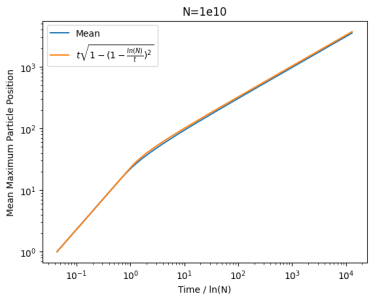
\includegraphics[width=8cm]{MaxMean1e10}
\caption{Mean maximum particle distance for $\beta$=1 with 1e10 particles.}
\label{fig:Mean}
\end{figure}

\subsubsection{Variance of the Maximum Particle Distance}
\indent\indent The variance of the distance has three major scaling regimes. It begins by scaling in powers of $t^{1/3}$, then $t^{1/2}$ and finally linear in $t$ as seen in Figure \ref{fig:Variance}. We see scaling proportional to $t$ at long times since the particles are effectively so far apart that the maximum particle undergoes a random walk. We should define somehow where the regimes are valid I think.

\begin{figure}[H]
\centering
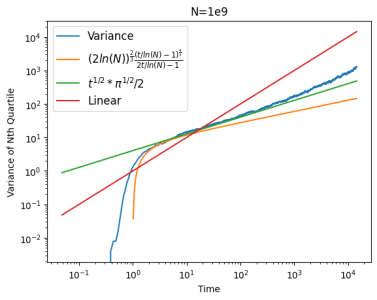
\includegraphics[width=8cm]{Var1e9}
\caption{Variance of 1e9 quantile for 1e10 particles and $\beta=1$. I think the x-axis might actually be time/lnN.}
\label{fig:Variance}
\end{figure}

\subsection{Quantiles}
\indent\indent To measure the quantiles our system we need to construct the PDF of an environment. We do this by using the recursion relation below to find the probability at each position x at time t

\begin{equation}
p_{B}(x, t) = p_{B}(x-1, t-1)B_{x-1, t-1} + p_{B}(x+1, t-1)(1 - B_{x+1, t-1})
\end{equation}

where $p_{B}(x,t)$ is the probability at position x at time t and $B_{x, t}$ is the probability of moving right. We initialize the system with all the particles starting at position zero so $p_{B}(x=0, t=0) = 1$. This differs from the physical system in that we aren't randomly moving particles left/right so there is another element of randomness that is missing from the PDF. However, the PDF provides an approach to capture most of the behaviour of the physical system. We will measure the mean and variance of the quantiles over many environments as seen below.

\subsubsection{Distributions}
\indent\indent Recall there were threme major regimes that we used to approximate the variance of the system as seen in Figure \ref{fig:Variance}. The first regime was for $t~lnN$ and relies on the Tracy-Widom distribution. The second regime was for $t~lnN^2$ and relies on the solution to the KPZ equation. The third and final regime was when all the particles broke up so much that the maximum particle is undergoing a random walk (Einstein Diffusion). This occurs at about $t~lnN^2.5?$.

\subsubsection{The TW Regime ($t~lnN$)}
\indent\indent The method used to derive the variance of the maximum particle relies on finding quantiles of the environment's PDF. Another formulation is to measure the probability a particle is above some position $x=vt$ where $v$ is a velocity between 0 and 1. We will write the probability of being above position x at time t as $P_{B}(x,t)$. Our theoretical predictions give us

\begin{equation}
ln(P_{B}(x, t)) = -It + t^{\frac{1}{3}}\sigma M
\end{equation}

where I = (insert equation here), $\sigma=(insert equation here)$, and M is the mean of the TW distribution.

\begin{figure}[H]
\centering
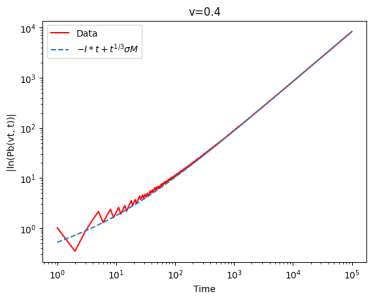
\includegraphics[width=8cm]{Mean0_4}
\caption{Mean $ln(P_{B}(v, t)$ over time for v=0.4}
\label{fig:MeanVelocity}
\end{figure}

We also have the prediction for the variance as

\begin{equation}
ln(P_{B}(x, t)) = t^{\frac{2}{3}}\sigma^{2}V
\end{equation}

where V is the variance of the TW distribution.

\begin{figure}[H]
\centering
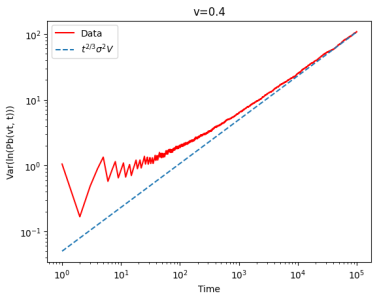
\includegraphics[width=8cm]{Var0_4}
\caption{Variance of $ln(P_{B}(v, t)$ over time for v=0.4}
\label{fig:VarVelocity}
\end{figure}

\indent For long times both the mean and variance appear to match the theory well as seen in Figures \ref{fig:MeanVelocity} and \ref {fig:VarVelocity}. However, I think that showing these plots may be opening up a lot of questions. First off, for what times and velocities are these equations a good approximation. I think previously we saw that for v < 0.3 at t~100,000 the approximation broke down. If we show these plots I think we need to quantify exactly where they are valid. This may come back to looking at the mean/variance as a function of velocity at several times. I'm not sure this will even be sufficient b/c we also need to say at what times these are valid.

\subsection{ToDo}

\begin{itemize}
	\item Look at simulations for the linear regime. Should be ending sometime soon (hopefully).
	\item Look at $P_{b}(vt^{3/4}, t)$ and see if we recover the solution to the KPZ equation
	\item Measure first time of arrival for various quantiles
	\item Discrete variance from PDF and CDF
	\item Plot velocities graphs all together. See if they collapse or something.
  \item Look at 10*N - 0.1*N to see if it follows the Gumbel distribution
\end{itemize}

\end{document}
